\section{Molecules}

\subsection{Ground State Energies}
 
\begin{table}
\begin{center}
\begin{tabular}{lrccrlrrc}
Molecule & $R$ & & \qquad & $E_\mathrm{VMC}$ & & \qquad $E_\mathrm{DMC}$ & \qquad\,\, Expt. & \qquad $\epsilon_\mathrm{rel}$\\
\hline\hline
\ \\
$\mathrm{H_2}$ & 1.4   & &\qquad & -1.1551(3)    & \qquad   & -1.1745(3)   & \qquad $-1.1746$      & \qquad $8.51\cdot 10^{-5}$ \\
\ \\
$\mathrm{Li_2}$& 5.051 & &\qquad & -14.743(3)    & \qquad   & -14.988(2)   & \qquad $-14.99544$    & \qquad $4.96\cdot 10^{-4}$ \\
\ \\
$\mathrm{Be_2}$& 4.63  & &\qquad & -28.666(5)    & \qquad   & -29.301(5)   & \qquad $-29.33854(5)$ & \qquad $1.28\cdot 10^{-3}$  \\
\ \\
$\mathrm{B_2}$ & 3.005 & &\qquad & -47.746(7)    & \qquad   & -49.155(5)   & \qquad $-49.4184$     & \qquad $5.33\cdot 10^{-3}$  \\
\ \\
$\mathrm{C_2}$ & 2.3481& &\qquad & -72.590(8)    & \qquad   & -74.95(1)    & \qquad $-75.923(5)$   & \qquad $1.28\cdot 10^{-2}$  \\
\ \\
$\mathrm{N_2}$ & 2.068 & &\qquad & -102.78(1)    & \qquad   & -106.05(2)   & \qquad $-109.5423$    & \qquad $3.19\cdot 10^{-2}$  \\
\ \\
$\mathrm{O_2}$ & 2.282 & &\qquad & -143.97(2)    & \qquad   & -148.53(2)   & \qquad $-150.3268$    & \qquad $1.2\cdot 10^{-2}$  \\
\ \\
\end{tabular}
\caption{Ground state energies for homonuclear diatomic molecules calculated using Variational - and Diffusion Monte-Carlo. The distance between the atoms $R$ are taken from Ref. \cite{H_He_exact} for $\mathrm{H_2}$ and from Ref. \cite{UmrigarMolecules} for $\mathrm{Li_2}$ to $\mathrm{O_2}$. The experimental energies are taken from Ref. \cite{H_He_exact} for $\mathrm{H_2}$ and from Ref. \cite{ExactMolecules} for $\mathrm{Li_2}$ to $\mathrm{O_2}$. As expected DMC is close to the experimental energy compared to VMC. $\epsilon_\mathrm{rel} = |E_\mathrm{DMC} - \mathrm{Expt.}|/|\mathrm{Expt.}|$}
\label{tab:MoleculesRes}
\end{center}
\end{table}


\begin{figure}
 \begin{center}
   \subfigure{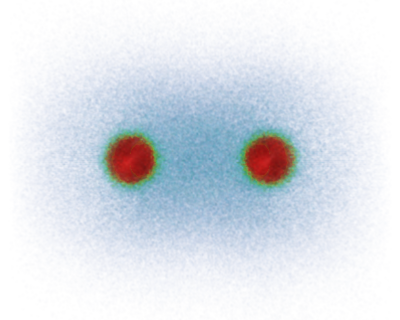
\includegraphics[scale=0.46]{../Graphics/OBD/OBD_MOL/Li2_3D.png}} 
   \subfigure{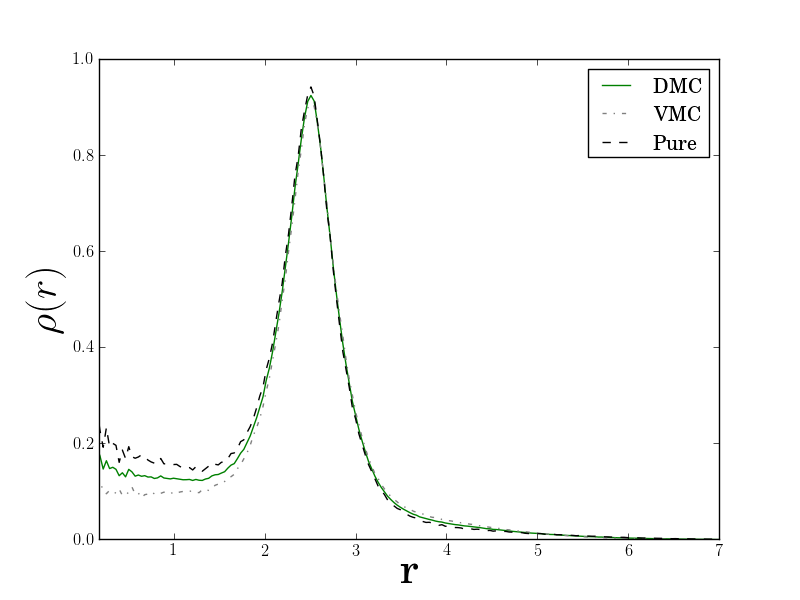
\includegraphics[scale=0.33]{../Graphics/OBD/OBD_MOL/Li2_2D.png}}  \\
   \subfigure{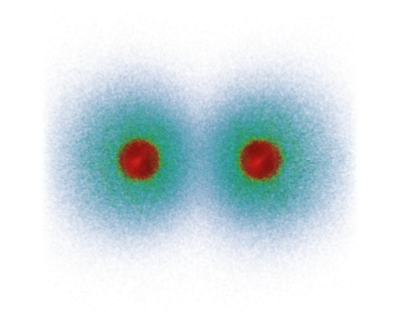
\includegraphics[scale=0.46]{../Graphics/OBD/OBD_MOL/Be2_3D.png}} 
   \subfigure{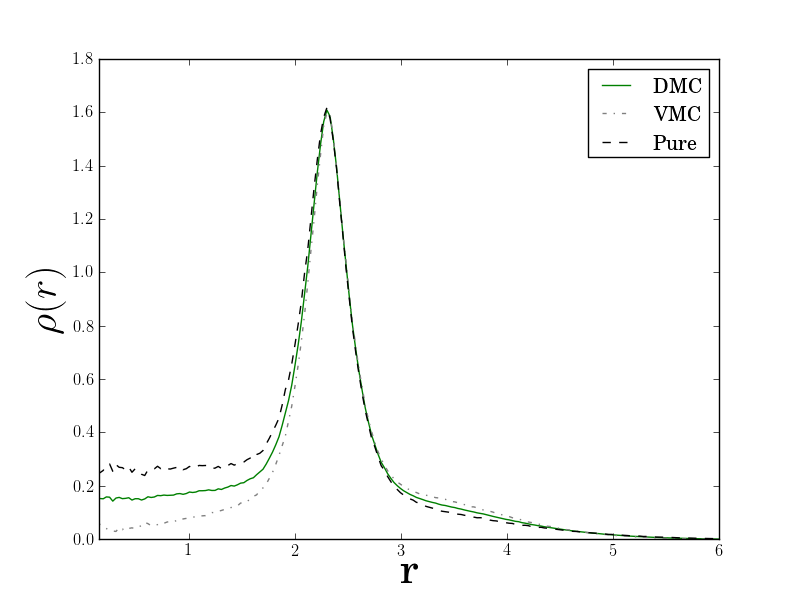
\includegraphics[scale=0.33]{../Graphics/OBD/OBD_MOL/Be2_2D.png}}  \\
   \subfigure{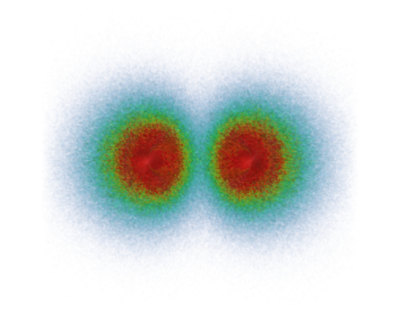
\includegraphics[scale=0.46]{../Graphics/OBD/OBD_MOL/O2_3D.png}} 
   \subfigure{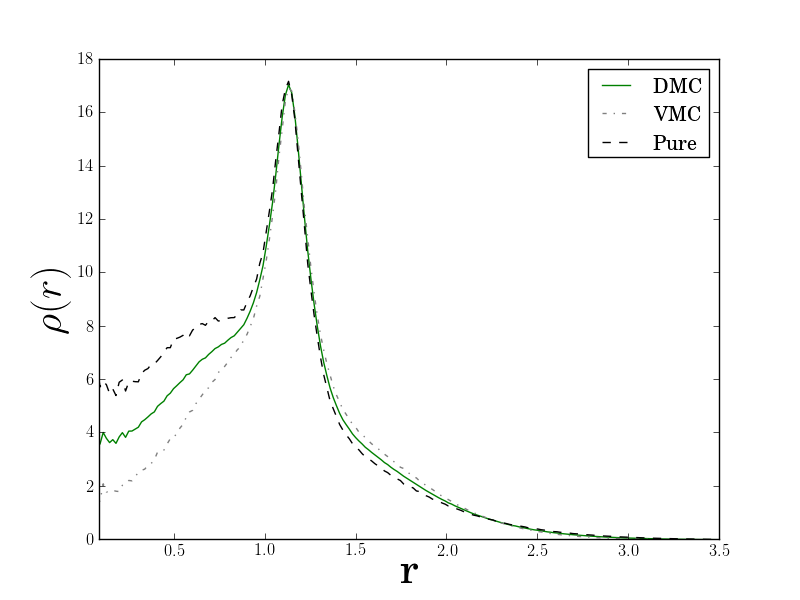
\includegraphics[scale=0.33]{../Graphics/OBD/OBD_MOL/O2_2D.png}}
  \caption{One-body densities for $\mathrm{Li_2}$ (top), $\mathrm{Be_2}$ (middle) and $\mathrm{O_2}$ (bottom). The figures on the left are 3D densities sliced through the middle, whereas the figures on the left are the radial one-body densities projected on the $x$-axis, i.e. the axis between the atoms. Red and blue color indicates a high and low electron density respectively. The left-hand figures are symmetric around the origin.}
  \label{fig:OBD_Molecules}
 \end{center}
\end{figure}



\begin{figure}
 \begin{center}
  \subfigure{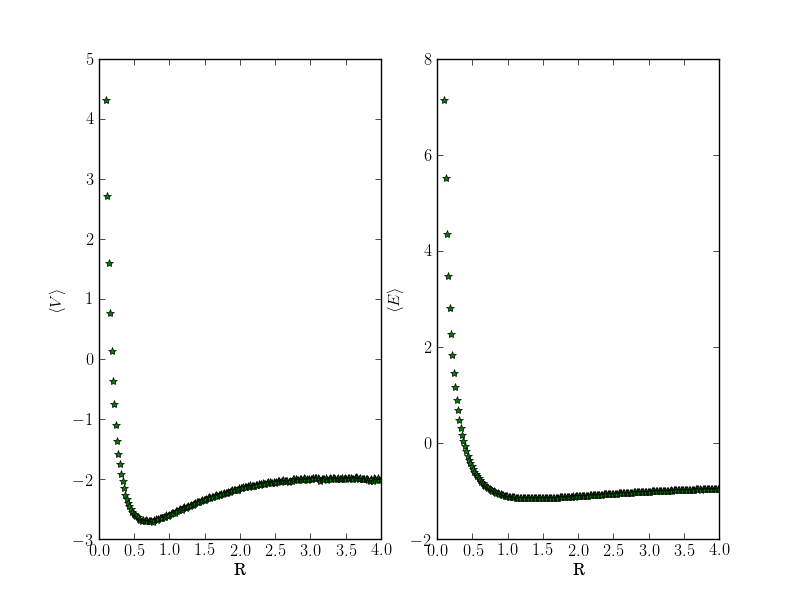
\includegraphics[scale=0.37]{../Graphics/R_VS_E/R_vs_E_hyd_0.png}}
  \subfigure{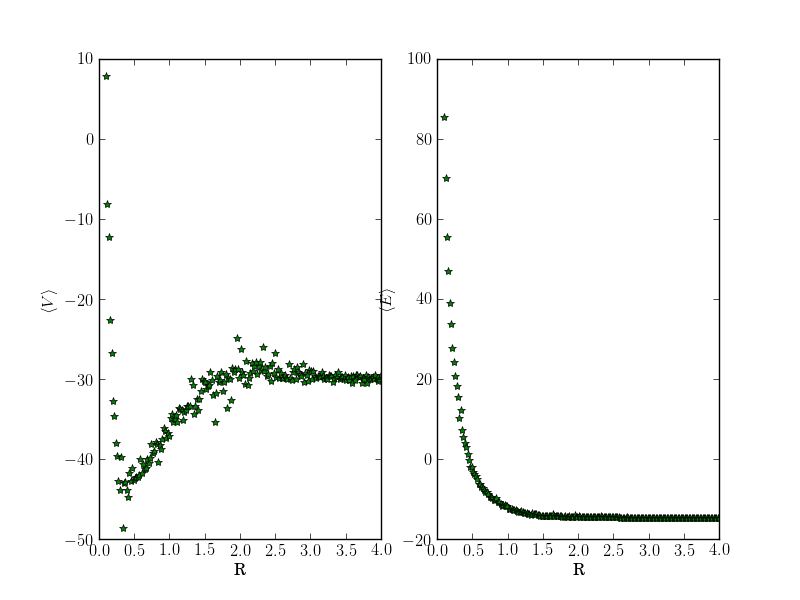
\includegraphics[scale=0.37]{../Graphics/R_VS_E/R_vs_E_lit_0.png}} 
  \caption{The distance between the atoms $R$ plotted against the potential and total energy for hydrogen gas (left) and litium gas (right). It is evident that there exist a well-defined minima in the energy in the case of hydrogen gas. For litium this is not the case, which corresponds well with the fact that litium does not appear naturally in a gas phase in nature.}
  \label{fig:molecules_R_vs_E}
 \end{center}
\end{figure}
